In this chapter we consider the properties and relationships between properties of a pure substance (such as water) which can exist in three phases – solid, liquid and gas. We will not consider the solid phase in this course.

As you read through this chapter, you will notice that we always define a state through two properties.  Based on the state postulate, this is sufficient to fully define the state.  In other words, all properties of a state can be found, provided we know at least two.
\newpage
%--------------------------------------------------------------------
\section{Phase Change and Property Diagrams}
%--------------------------------------------------------------------
In order to introduce the rather complex phase change interactions that occur in pure substances we consider an experiment in which we have liquid water in a piston-cylinder device at 20°C and 100kPa pressure. Heat is added to the cylinder while the pressure is maintained constant until the temperature reaches 300°C, as shown the $T$-$v$ diagram (temperature vs. specific volume) in Figure \ref{fig:ch2_TvDiagram}.

\begin{figure}[H]
\centering
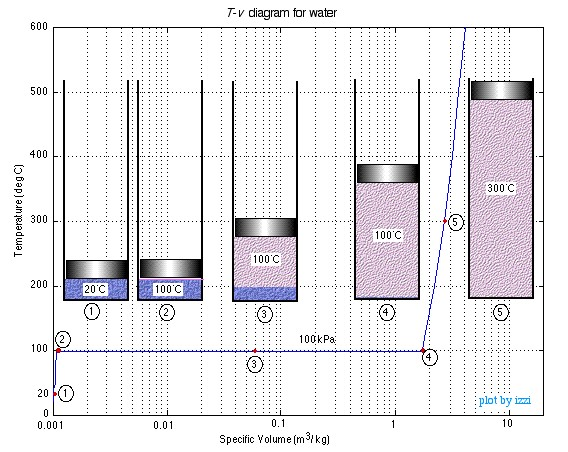
\includegraphics[width=0.9\textwidth]{TvDiagramForWater}
\caption{Heat is added to water at constant pressure, leading to boiling and an increase of volume.}
\label{fig:ch2_TvDiagram}
\end{figure}

From State (1) to State (2) the water maintains its liquid phase and the specific volume increases very slightly until the temperature reaches close to 100°C (State (2) – {\bf saturated liquid}). As more heat is added the water progressively changes phase from liquid to water vapor (steam) while maintaining the temperature at 100°C ({\bf saturation temperature} – $T_{sat}$) until there is no liquid remaining in the cylinder (State (4) – {\bf saturated vapor}). If heating continues then the water vapor temperature increases ($T > T_{sat}$) and is said to be {\bf superheated} (State (5)).

Notice that during this entire process the specific volume of the water increased by more than three orders of magnitude, which made it necessary to use a logarithmic scale for the specific volume axis.

This first experiment was performed at constant pressure.  If we increased the force on the piston (perhaps by increasing the mass of the piston), we could increase the pressure in the system.  Then, we could cool the system until it was a liquid, and repeat the experiment again. Figure \ref{fig:ch2_TvDiagram2} contains data from four such experiments, at 100 kPa, 1 MPa, 10 MPa, and 22 MPa.

\begin{figure}[H]
\centering
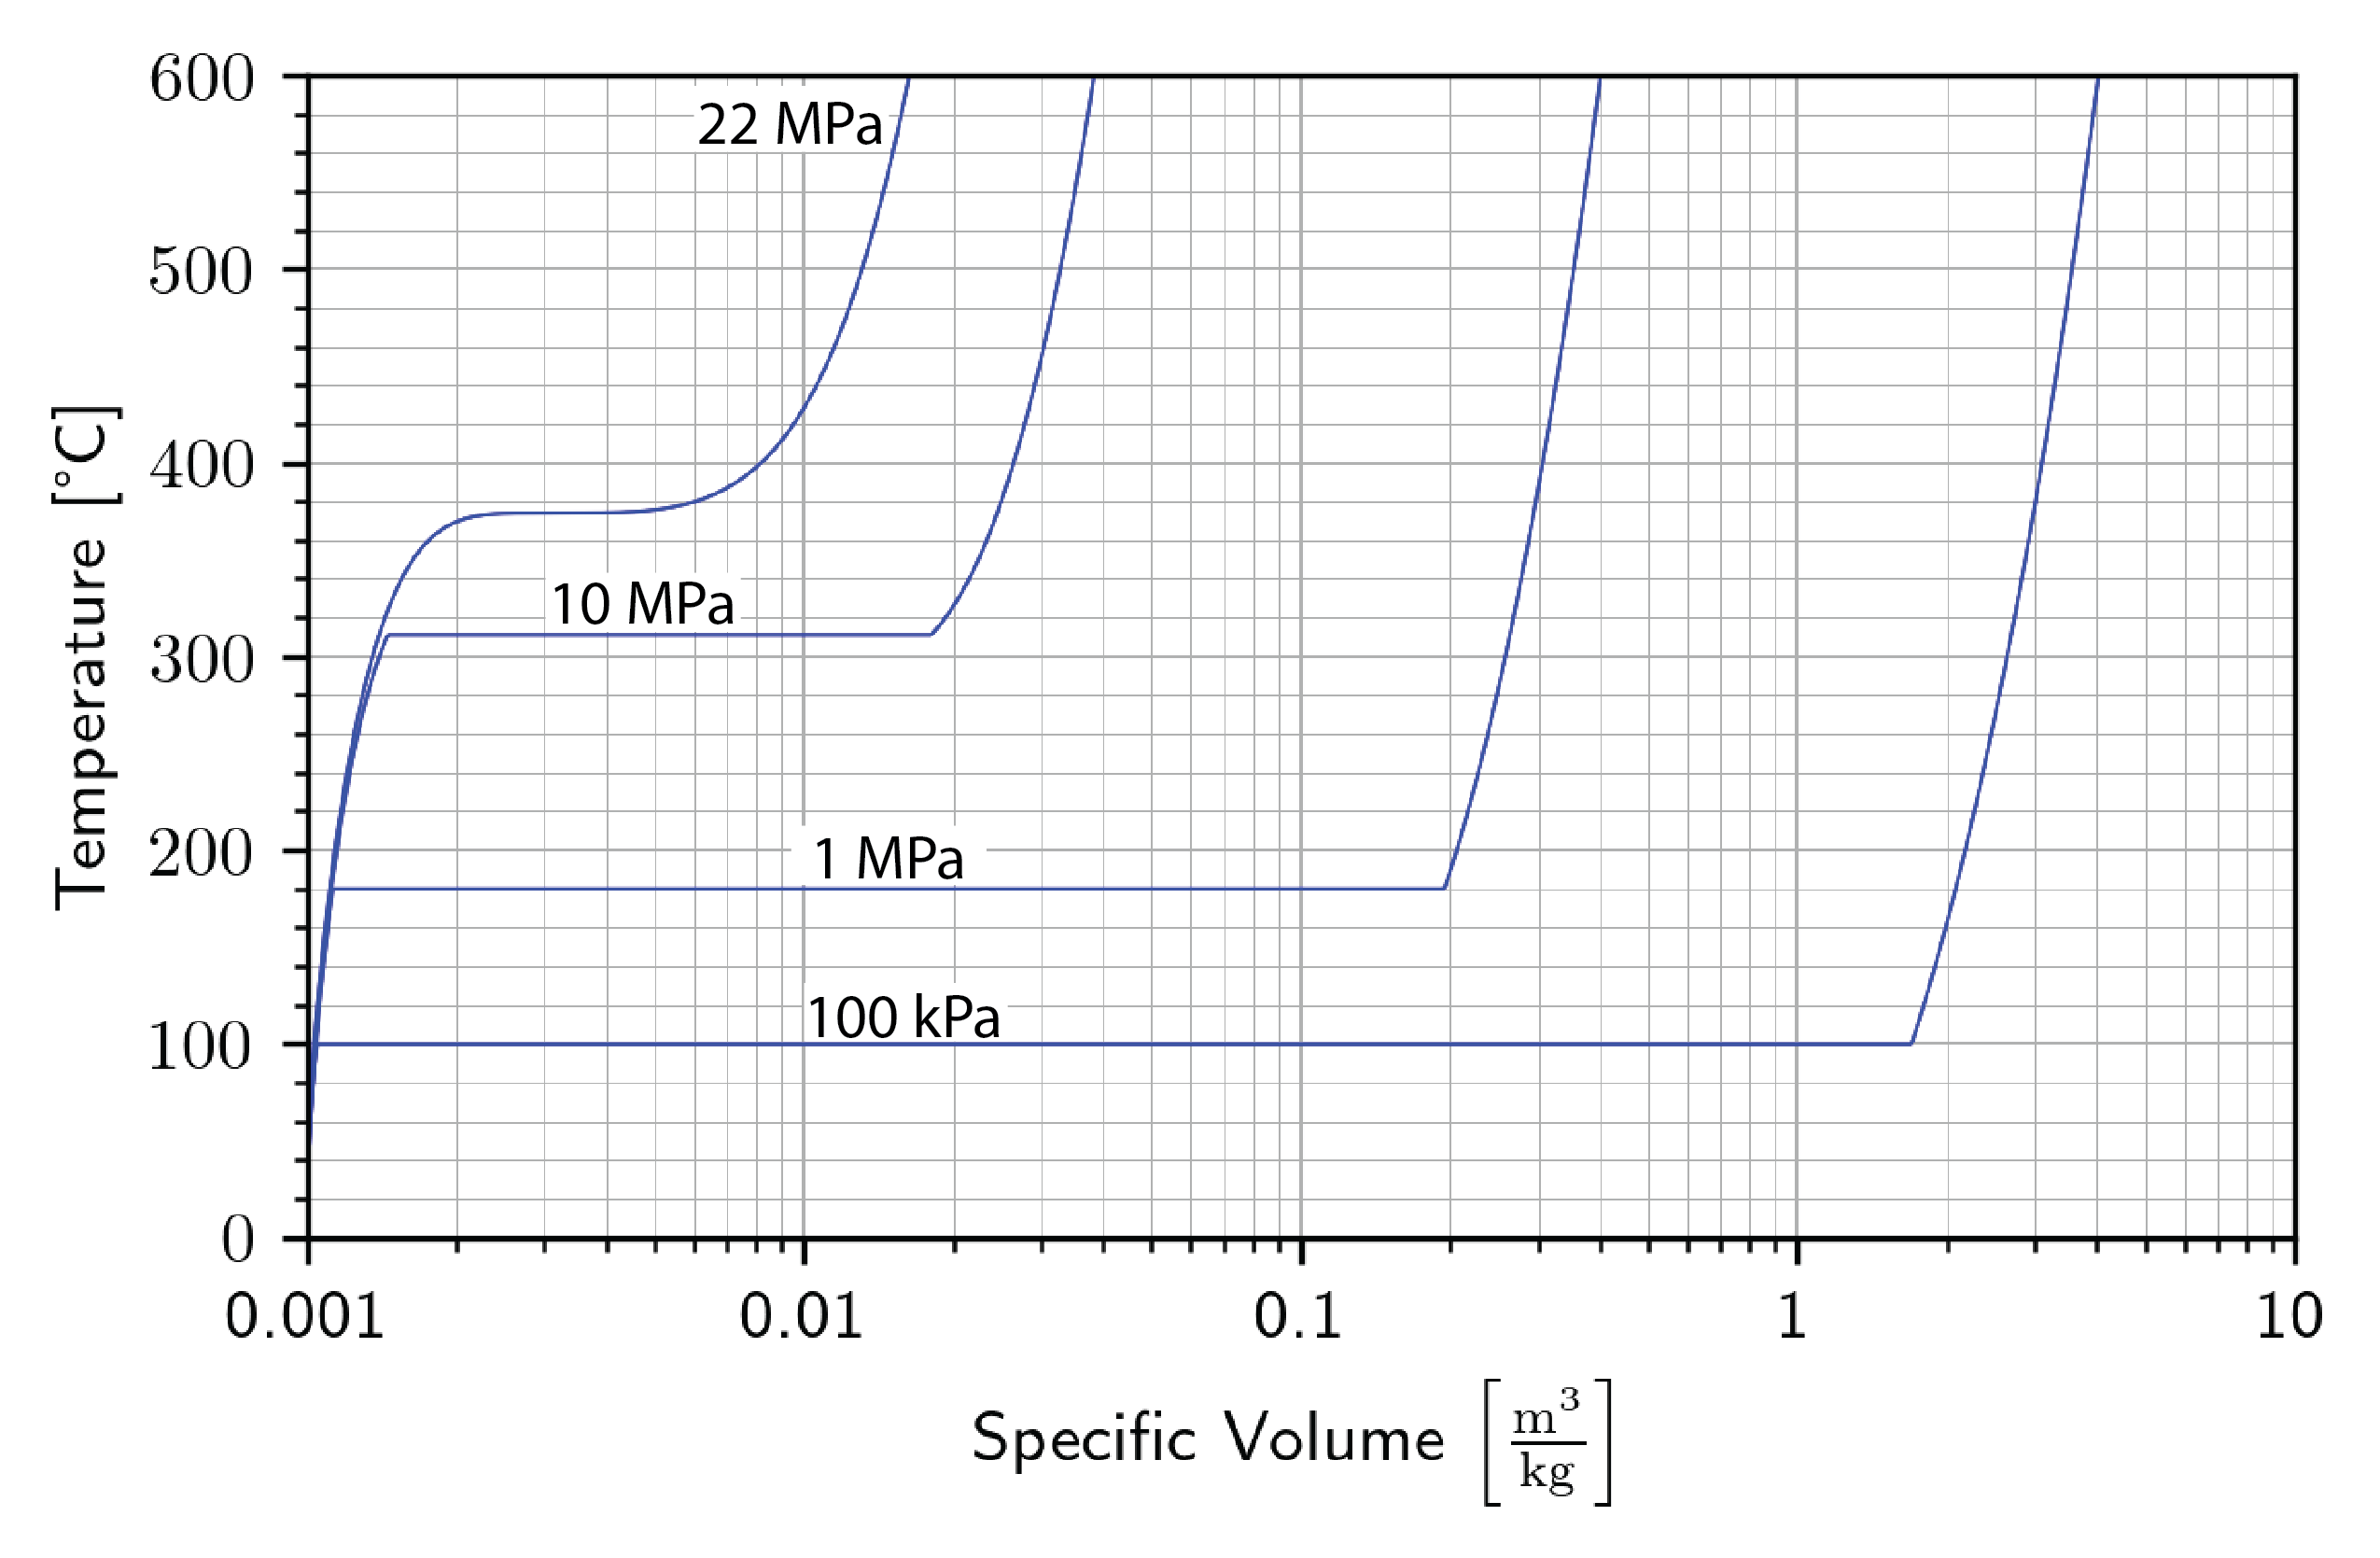
\includegraphics[width=0.9\textwidth]{isobars}
\caption{Heat is added to water at multiple pressures.}
\label{fig:ch2_TvDiagram2}
\end{figure}

As the pressure increases, the constant temperature region between saturated liquid and saturated vapor becomes smaller and smaller until it is eliminated completely at the critical point.  Above the critical point, there is no clear distinction between the liquid and vapor states.

Fluids with temperatures above the {\bf critical temperature} are known as {\bf supercritical fluids} or {\bf superheated} fluids.  Increasing the pressure will cause the fluid to be more liquid-like, and decreasing the pressure will cause the fluid to be more gas-like. 

To help distinguish between the regions of the $T$-$v$ diagram, we separate the liquid, vapor, and liquid-vapor mixtures with {\bf saturation lines}.  These lines are drawn by noting each saturated liquid and saturated vapor points, and connecting them.  The end result is shown in Figure \ref{fig:ch2_TvDiagram3}.

\begin{figure}[H]
\centering
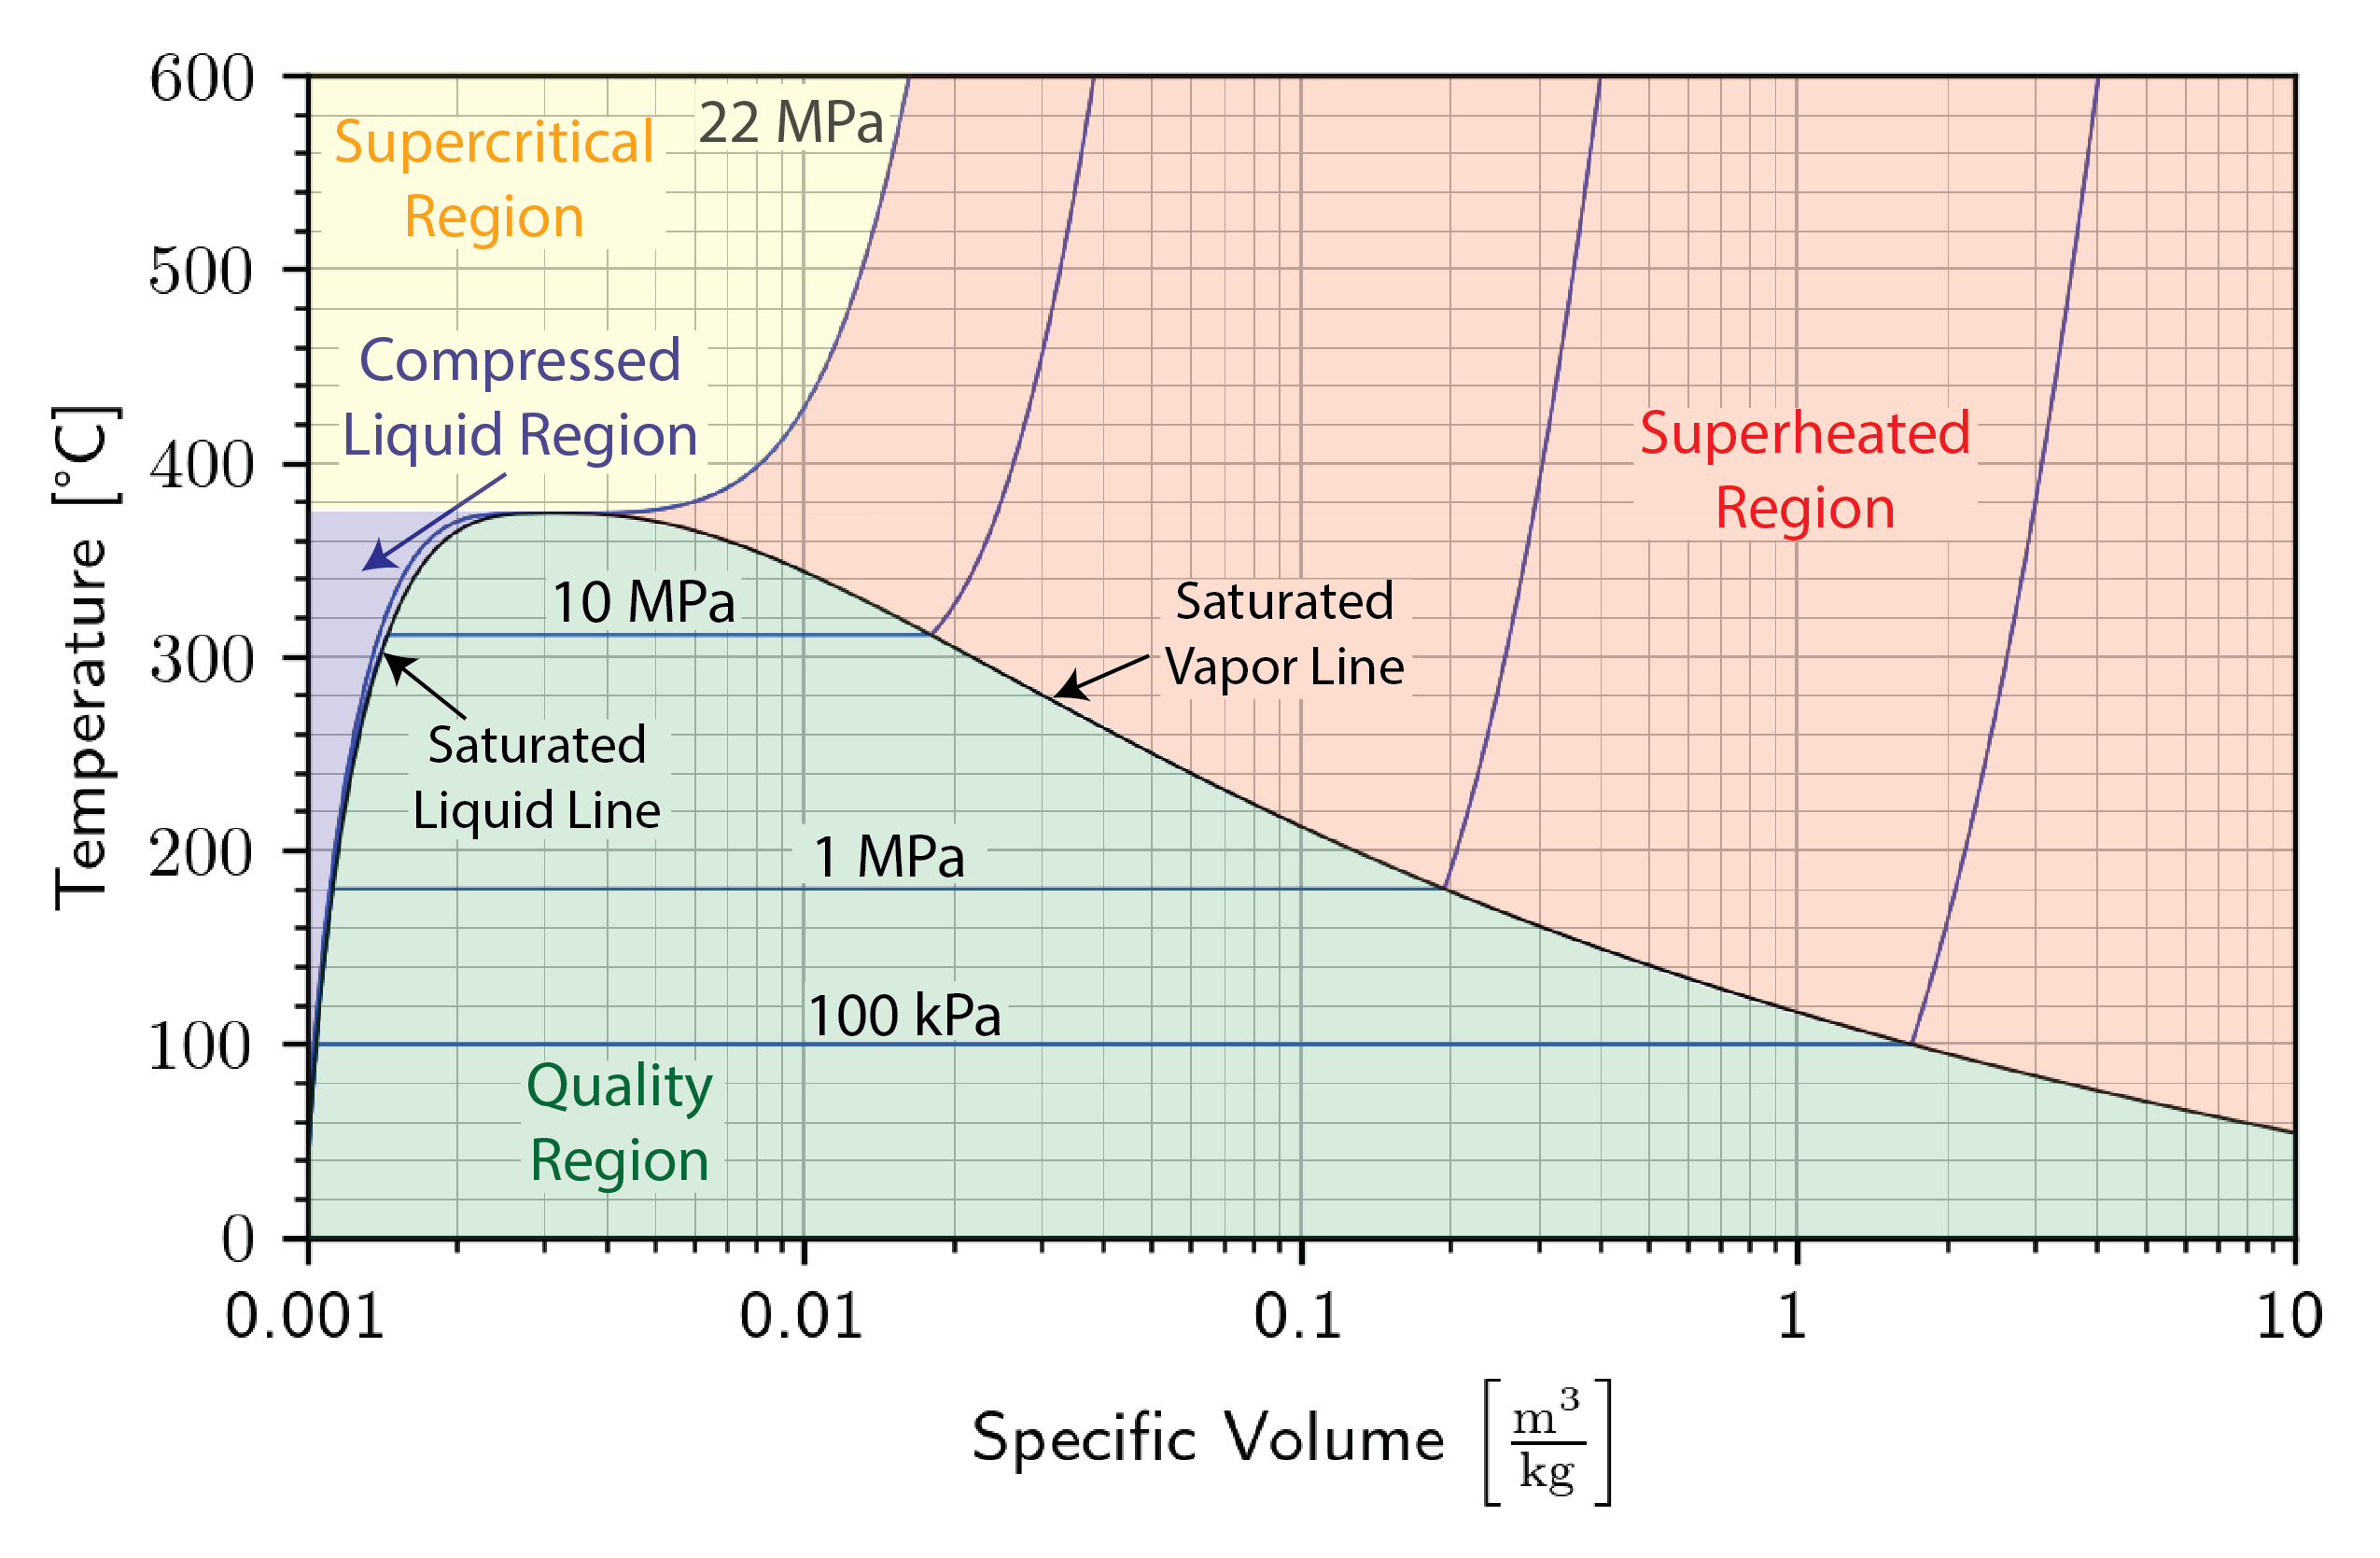
\includegraphics[width=0.9\textwidth]{TvDiagramWisobars}
\caption{$T$-$v$ diagram with saturation curves shown.}
\label{fig:ch2_TvDiagram3}
\end{figure}

The saturation lines define the regions of interest as shown in the diagram, being the {\bf compressed liquid} region to the left (blue), the {\bf quality} region or {\bf saturated} region enclosed by the saturation lines (green), and the {\bf superheated} region to the right of the saturated vapor line and critical pressure line (red), and the {\bf supercritical} region at temperatures and pressures higher than the critical point (yellow).

We will use {\bf property tables} associated with the regions in order to evaluate the various properties. Notice that we have provided property tables of steam and Refrigerant R134a in Appendix \ref{ch:appendixSteam} and \ref{ch:appendixR134a}.

\section{Quality}

The {\bf quality region}, also referred to as the {\bf saturated liquid-vapor mixture region}, is the area enclosed between the saturated liquid line and the saturated vapor line. At any point within this region the quality of the mixture (represented by the symbol $x$) is defined as the mass of vapor divided by the total mass of the fluid, as defined in Equation \ref{eq:quality}.
\begin{equation} \label{eq:quality}
  x = \frac{m_{\rm gas}}{m_{\rm total}}
\end{equation}

We can also use the {\bf rule of mixtures} to define mass-specific properties.  As an example, this is done for specific volume as follows:
\begin{align*}
  V &= V_f + V_g \\
  m v &= m_f v_f + m_g v_g \\
  m v &= (m-m_g) v_f + m_g v_g \\
  v &= \left(1 - \frac{m_g}{m}\right) v_f + \frac{m_g}{m} v_g \\
  v &= (1-x) v_f + x v_g
\end{align*}

Notice that properties relating to the saturated liquid have the subscript $f$, and those relating to the saturated vapor have the subscript $g$. If we consider a volume $V$ containing a mass $m$ of a saturated liquid-vapor mixture, we can calculate the quality $x$ as follows:

\begin{align}
  \nonumber v &= (1-x) v_f + x v_g\\
  \nonumber v &= v_f + x\left(v_g - v_f\right)\\
  \label{eq:quality2} x &= \frac{v - v_f}{v_g - v_f}
\end{align}

This is demonstrated graphically in Figure \ref{fig:ch2_TvDiagram4}.

\begin{figure}[H]
\centering
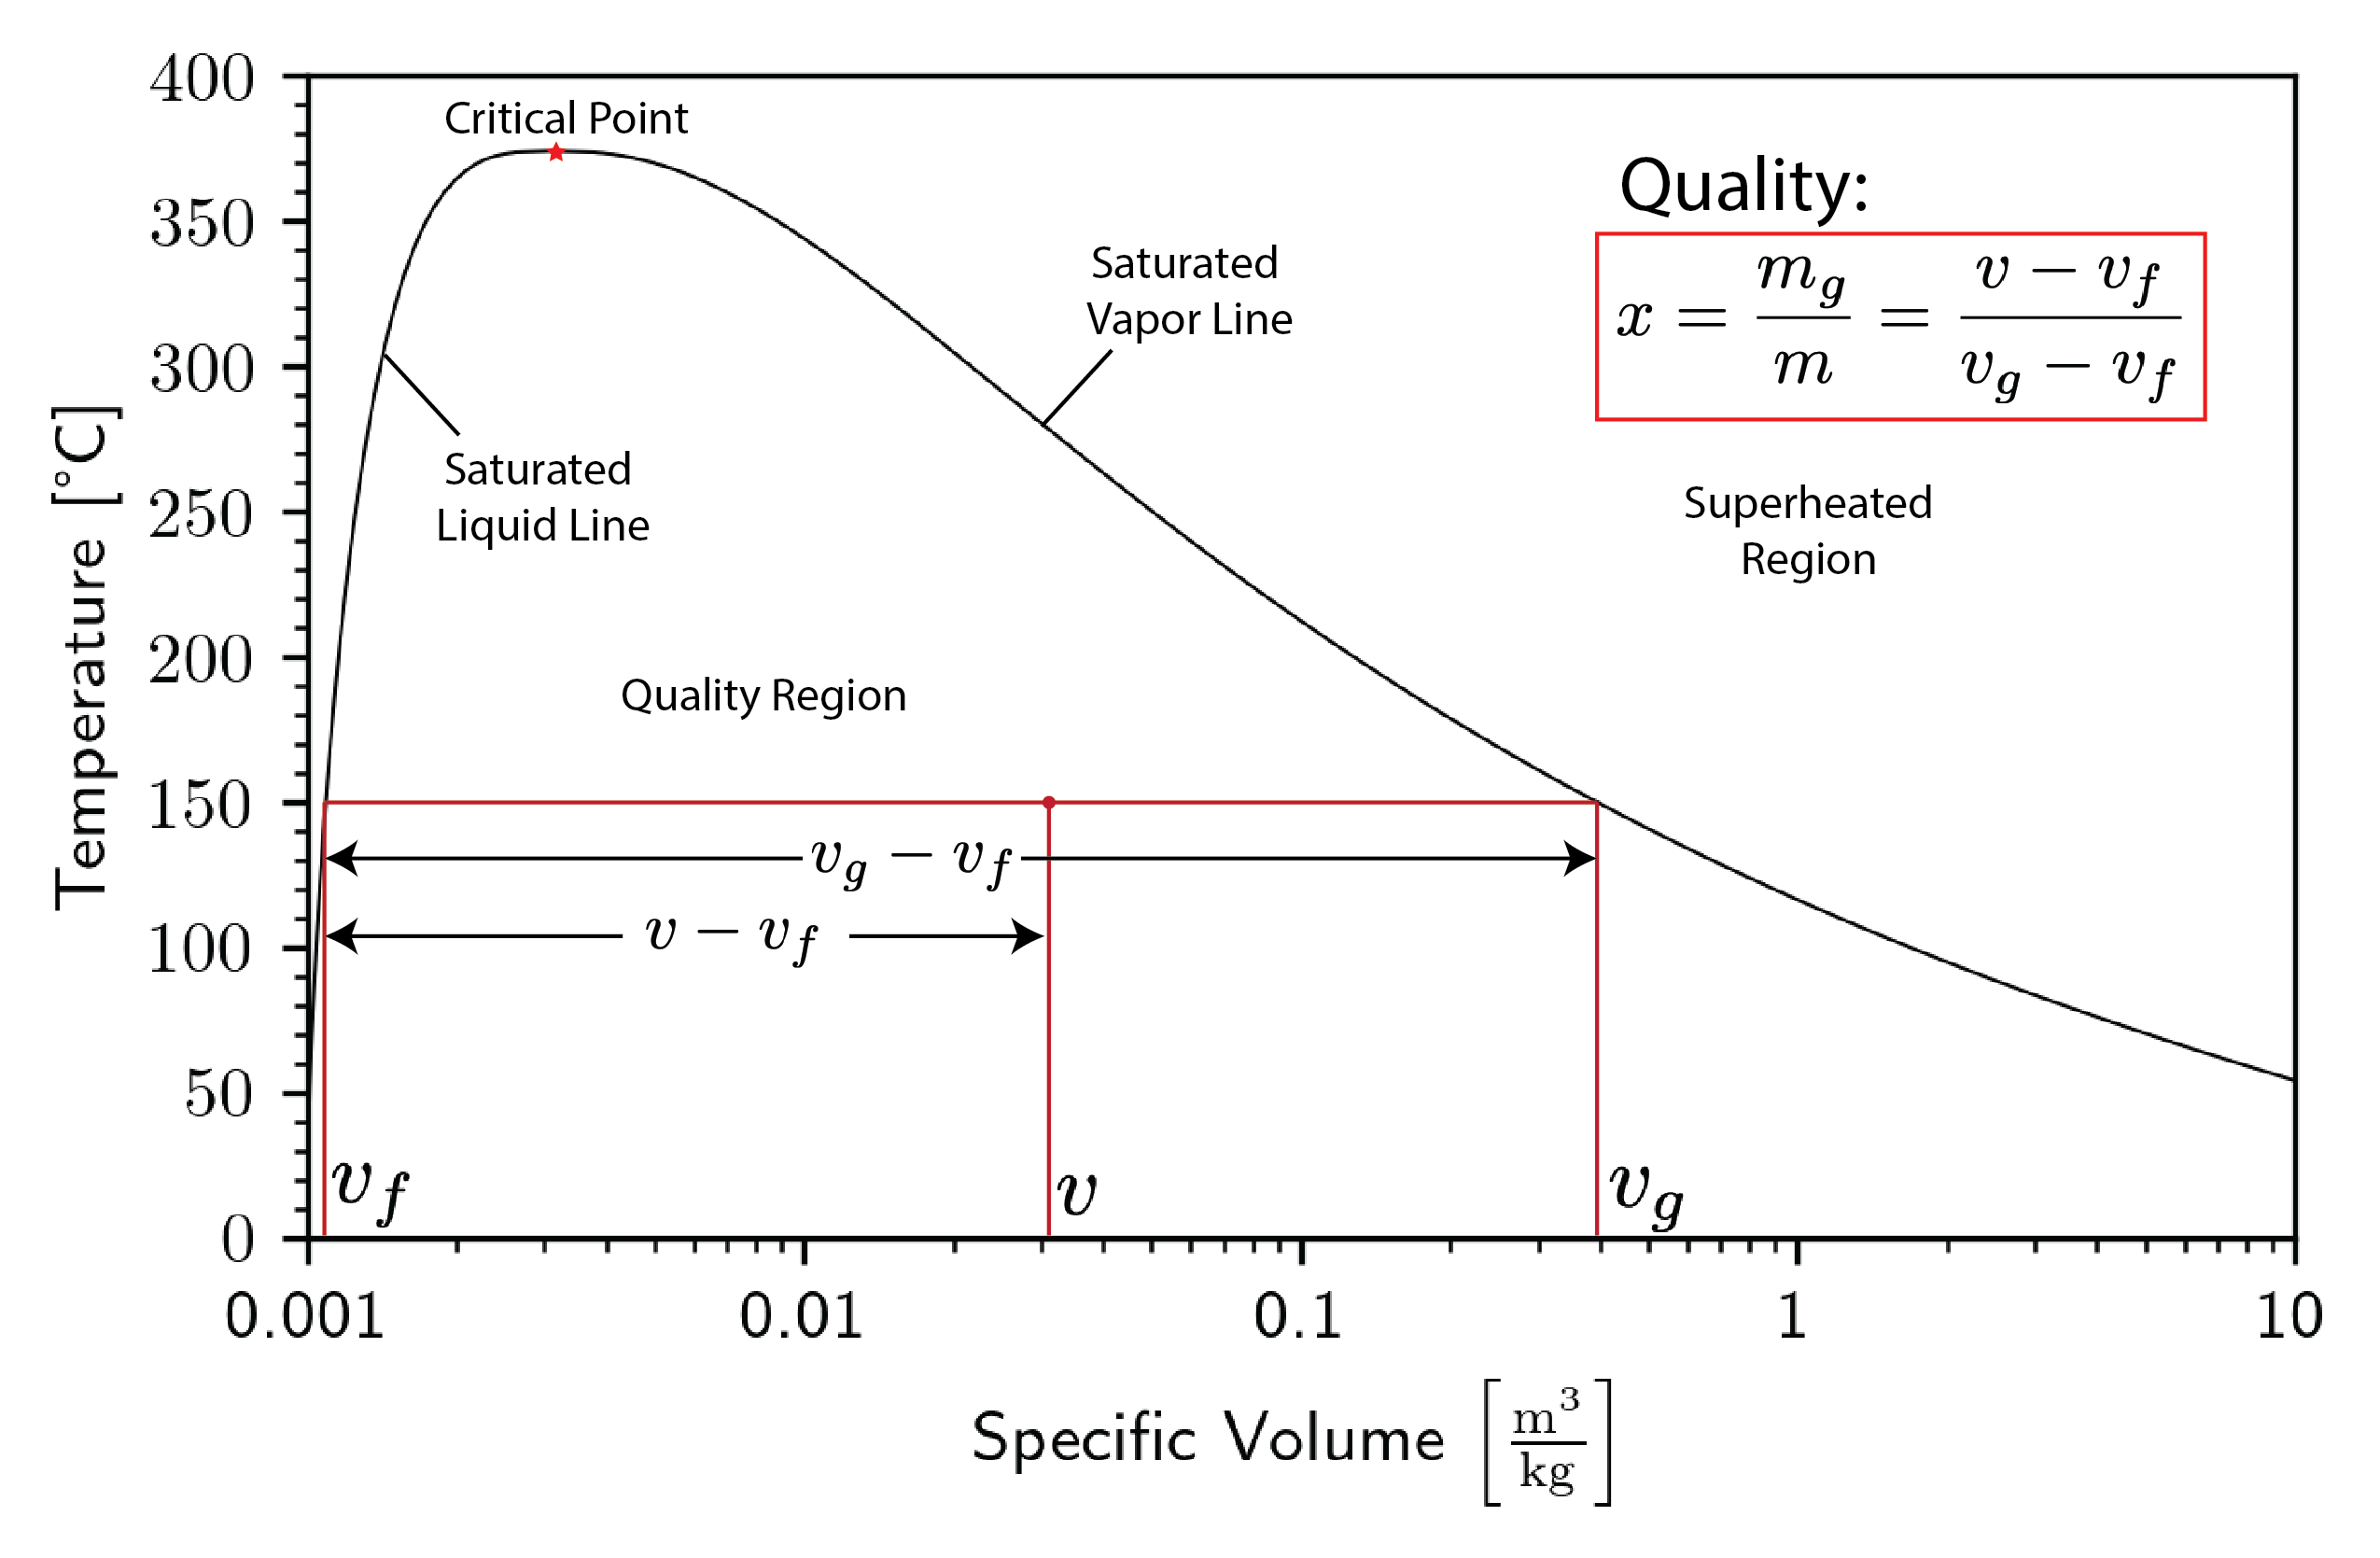
\includegraphics[width=1.0\textwidth]{TvDiagramQuality}
\caption{Quality is the ratio of the mass of gas to the total mass within the system.}
\label{fig:ch2_TvDiagram4}
\end{figure}

%% \begin{figure}[H]
%% \centering
%% 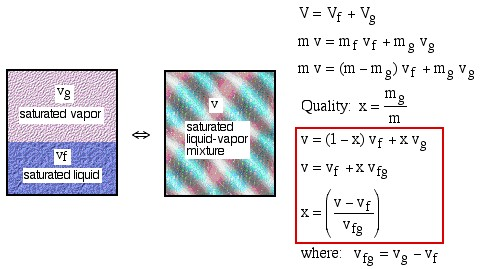
\includegraphics[width=0.75\textwidth]{VolumeEquations}
%% \caption{Quality can also be defined based on the specific volumes of the liquid ($v_f$) and gas ($v_g$).}
%% \label{fig:ch2_VolumeEquations}
%% \end{figure}

Typically, because of the extremely large range of specific volume values of interest, the $T$-$v$ diagram can only be done on a semi-log plot (logarithmic scaling on the $x$-axis). This is extremely inconvenient, so instead the $T$-$v$ diagram is normally not drawn to scale. Instead, it is only sketched in order to help define the problem, which is then solved in terms of the steam tables. This approach is illustrated in an example below.

\begin{example}{Boiling Water}
  Two kilograms of water at 25°C are placed in a piston cylinder device under 100 kPa pressure (state (1)). Heat is added to the water at constant pressure until the piston reaches the stops at a total volume of 0.4 m3 (state (2)). More heat is then added at constant volume until the temperature of the water reaches 300°C (state (3)). Determine (a) the quality of the fluid and the mass of the vapor at state (2), and (b) the pressure of the fluid at state (3).


{\bf Step 1: Diagram} \quad  \underline{Always} draw a complete diagram of the states and processes of the problem and include all the relevant information on the diagram. In this case there are three states and two processes (constant pressure and constant volume).

\begin{center}
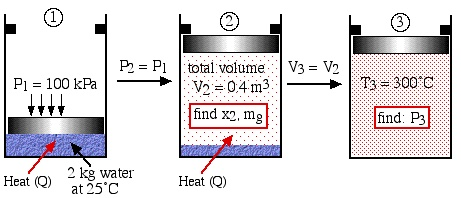
\includegraphics[width=0.75\textwidth]{example2-1}
%\captionof{figure}{}
%\label{fig:ch2_example1}
\end{center}

{\bf Step 2: $p$-$v$ or $T$-$v$} \quad  In the case of a closed system with a phase change fluid, always sketch a $T$-$v$ or $p$-$v$ diagram indicating all the relevant states and processes on the diagram. As mentioned above this diagram will not be drawn to scale, however it will help to define the problem and the approach to solution. In the case of steam, as we determine various values from the steam tables we add these values to the diagram, typically as shown below:

\begin{center}
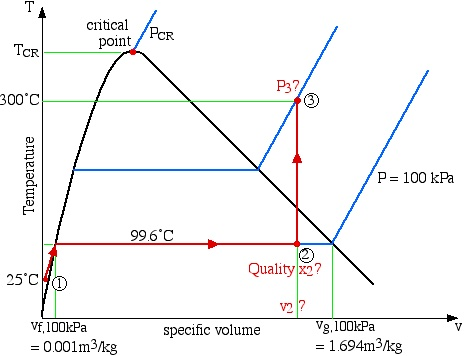
\includegraphics[width=0.6\textwidth]{example2-1_Tv}
%\captionof{figure}{}
%\label{fig:ch2_example1_Tv}
\end{center}


{\bf Step 3: Address Prompt} \quad Notice that the $T$-$v$ diagram is based exclusively on intensive properties, hence mass is not indicated on the diagram. Thus we indicate on the diagram that in order to determine the quality at state (2) we need to first evaluate the specific volume $v_2$, which can then be compared to the saturation values $v_f$ and $v_g$ at the pressure of 100 kPa.

Thus:
\begin{equation*}
  v_2 = \frac{V}{m} = \frac{0.4\ \rm m^3}{\rm 2\ kg} = 0.2 \frac{\rm m^3}{kg}
\end{equation*}

Quality can be found via Equation \ref{eq:quality2}:

\begin{equation*}
  x_2 = \frac{v_2-v_f}{v_g-v_f} = \frac{0.2 - 0.001}{1.694-0.001}\rightarrow \redbox{x_2 = 0.118}
\end{equation*}

Finally, the mass of water vapor:
\begin{equation*}
  x = \frac{m_g}{m_{tot}} \rightarrow m_{g_2} = x_2\cdot m_{tot} = 0.118 \cdot 2\ {\rm kg} \rightarrow \redbox{m_{g_2} = 0.235\ {\rm kg}}
\end{equation*}

Concerning state (3), the problem statement did not specify that it is in the superheated region. We needed to first determine the saturated vapor specific volume $v_g$ at 300°C. This value is 0.0216 $\rm m^3$/kg, which is much less than the specific volume $v_3$ of 0.2 $\rm m^3$/kg, thus placing state (3) well into the superheated region. Thus the two intensive properties which we use to determine the pressure at state (3) are $T_3$=300°C, and $v_3$=0.2 $\rm m^3$ / kg. On scanning the superheated tables we find that the closest values lie somewhere between 1.2 MPa and 1.4 MPa, thus we use linear interpolation techniques to determine the actual pressure $p_3$ as shown below:

\begin{center}
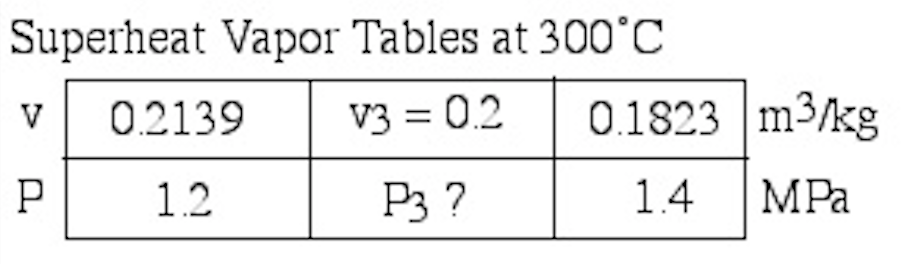
\includegraphics[width=0.5\textwidth]{example2-1_p3}
%\captionof{figure}{}
%\label{fig:ch2_example1_p3}
\end{center}

Linear interpolation has a good description from \href{https://en.wikipedia.org/wiki/Linear_interpolation}{Wikipedia}, but we will use it as follows:
\begin{equation*}
  \frac{\Delta p_A}{\Delta p_b} = \frac{\Delta v_A}{\Delta v_b} \rightarrow \frac{p_3 - 1.2}{1.4-1.2} = \frac{0.2-0.2139}{0.1823-0.2139} = 0.440
\end{equation*}

Therefore, $\redbox{p_3=1.29\ \rm MPa.}$

\end{example}

If you check the steam property tables, you will see that we have also included three new properties: internal energy $u$ [kJ/kg], enthalpy $h$ [kJ/kg], and entropy $s$ [kJ/kgK].  All of these will be defined as needed in future sections. At this stage we note that the 3 equations relating quality and specific volume can also be evaluated in terms of these three additional properties.

\begin{align*}
  u &= (1-x)\ u_f + x\ u_g \\
  h &= (1-x)\ h_f + x\ h_g \\
  s &= (1-x)\ s_f + x\ s_g
\end{align*}

% --------------------------------------------------------------------
\section{The $p$-$v$ Diagram for Water}
% --------------------------------------------------------------------
The above discussion was done in terms of the temperature ($T$) and specific volume ($v$). You may recall from Chapter 1 when we defined the State Postulate however, that any two independent intensive properties can be used to completely define all other intensive state properties. This means we can also evaluate a substance in terms of pressure ($p$) and specific volume ($v$) as shown below:

\begin{figure}[H]
\centering
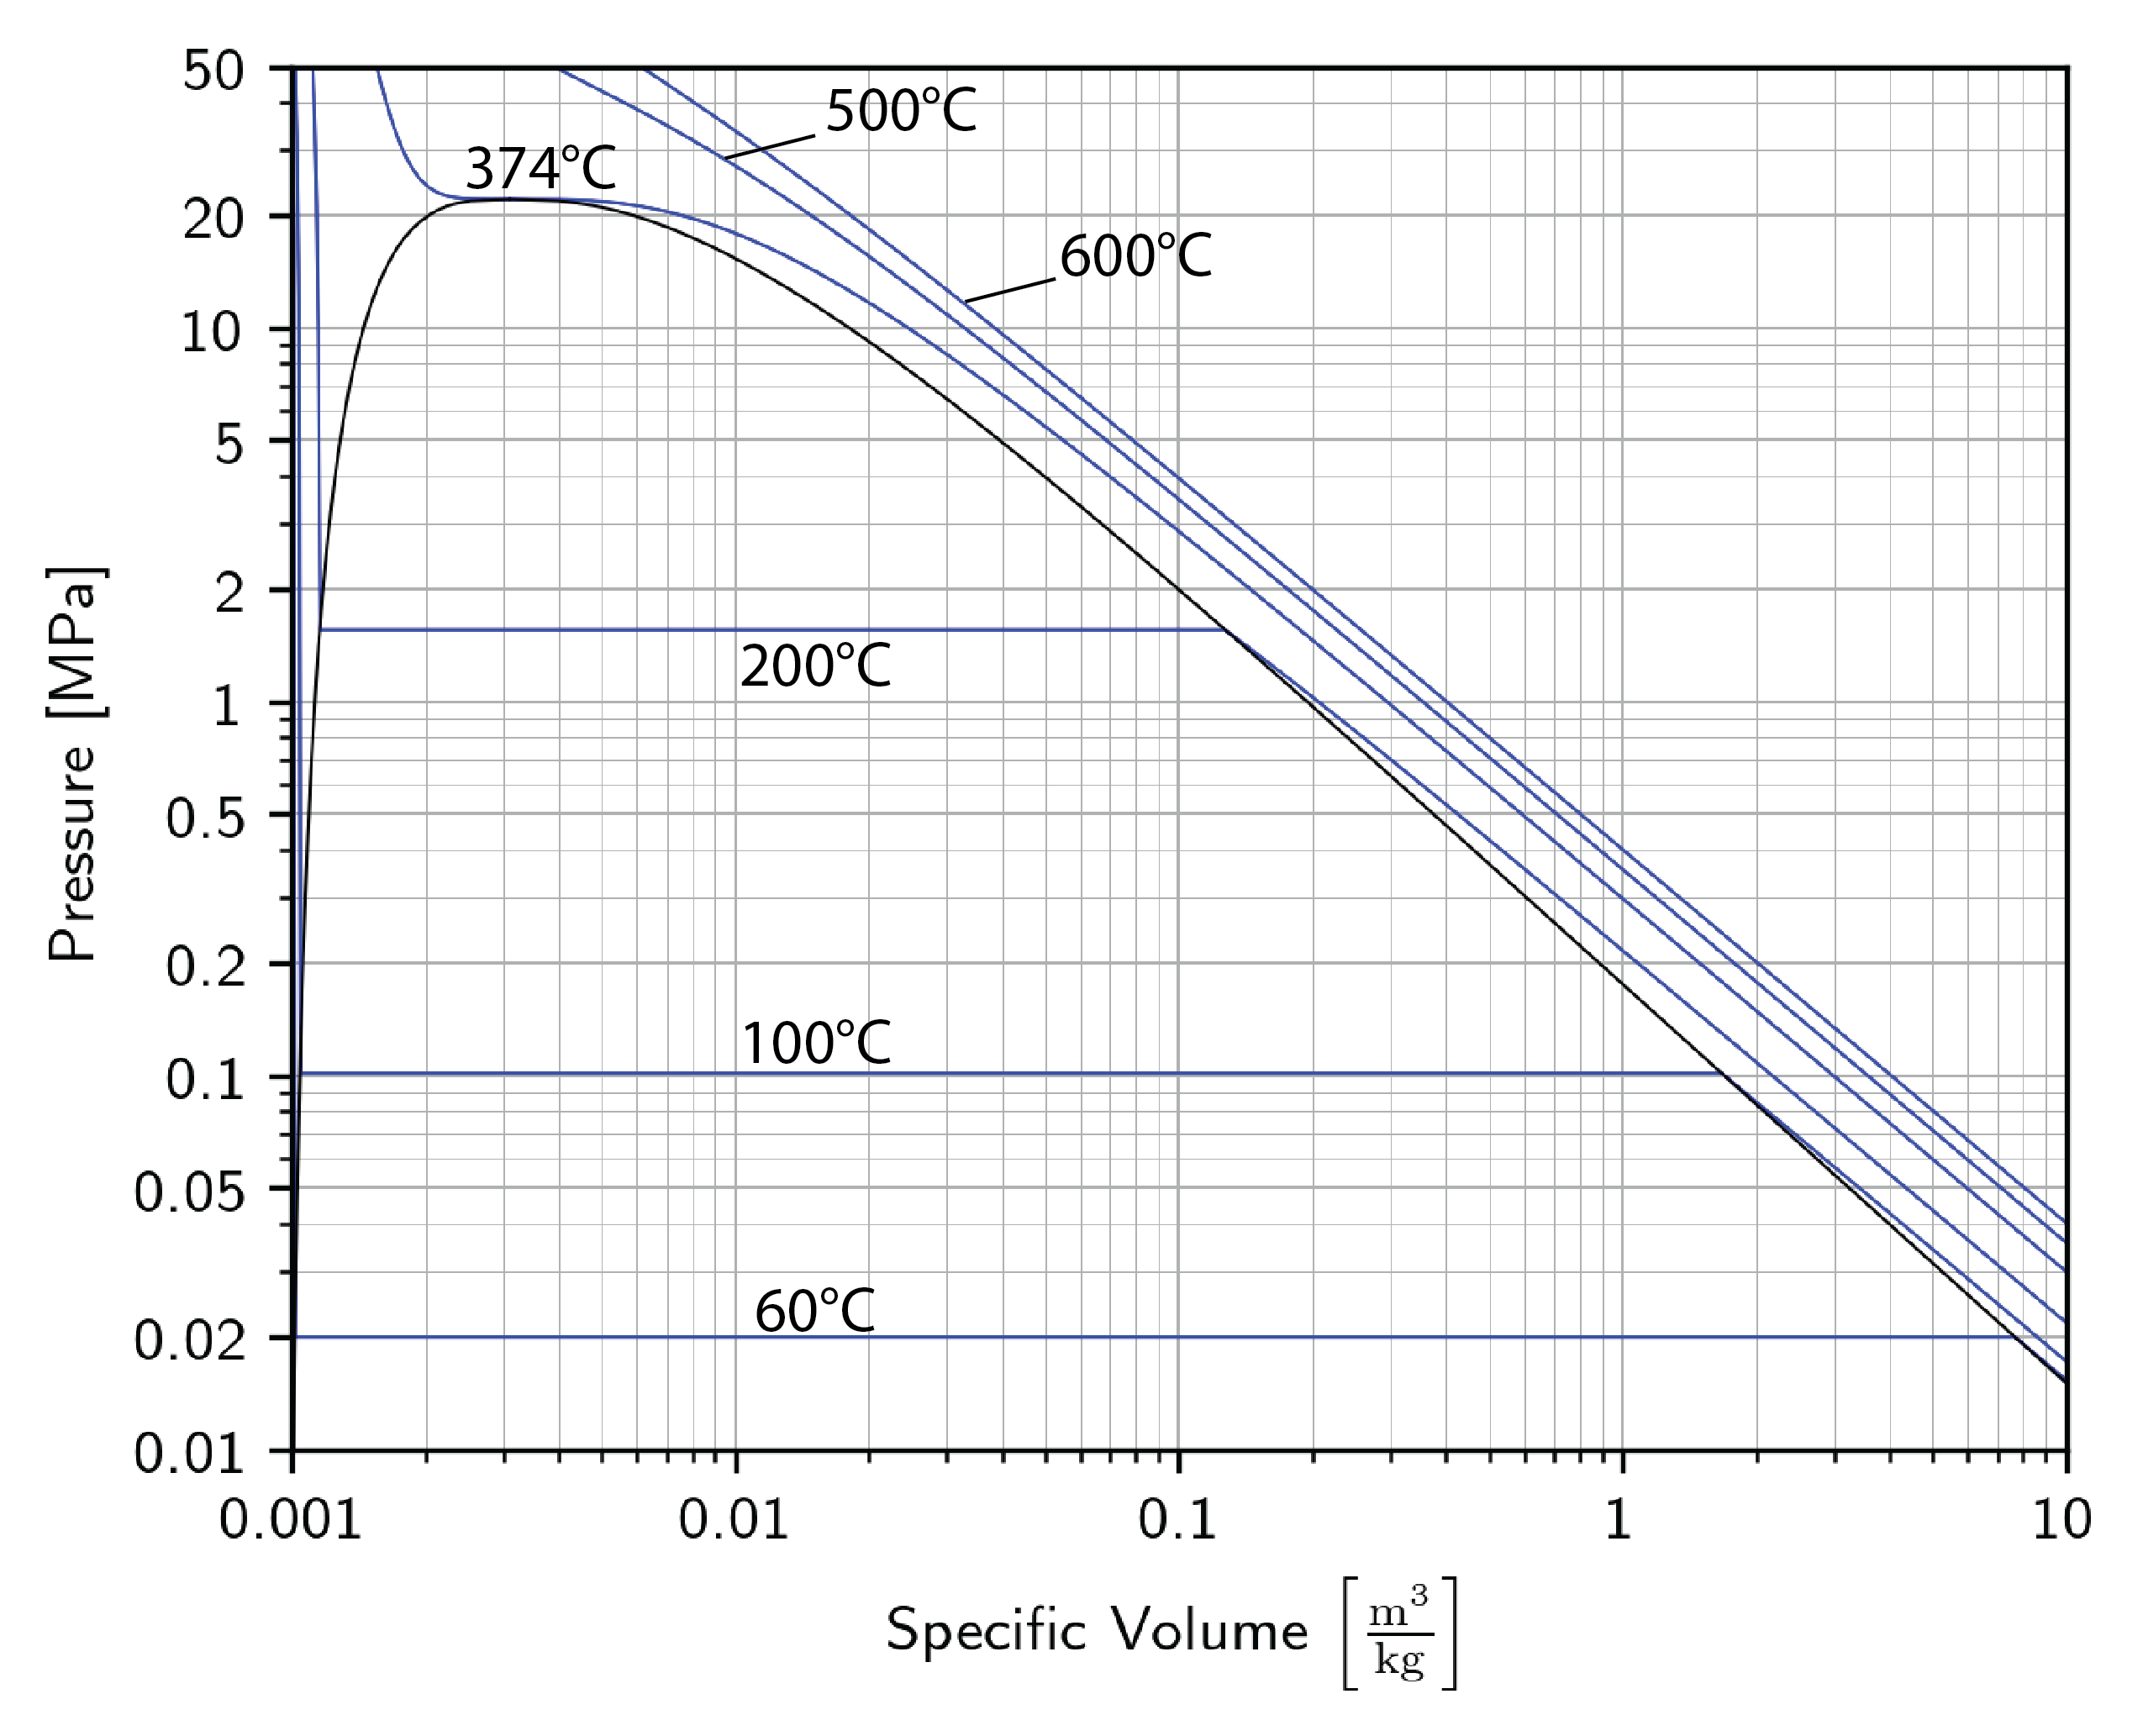
\includegraphics[width=0.75\textwidth]{pvDiagramWisothermal}
\caption{Variation of pressure and specific volume for water at various temperatures.  Note that both the x- and y- axes are logarithmic.}
\label{fig:ch2_PvDiagram}
\end{figure}

Similar to the $T$-$v$ diagram, we typically only sketch the $p$-$v$ diagram to solve problems, as seeing all relevant data requires a log-log plot.  Again, the example below illustrates this process.

\begin{example}[label={ex:ch2constantPressure}]{Constant Pressure Expansion}
  Two kilograms of water at 25°C are placed in a piston cylinder device under 3.2 MPa pressure as shown in the diagram (State (1)). Heat is added to the water at constant pressure until the temperature of the fluid reaches 350°C (State (2)). Determine the final volume of the fluid at state (2).

  {\bf Step 1: Diagram} \quad In this case, there are only two states.

\begin{center}
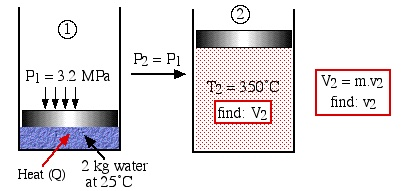
\includegraphics[width=0.6\textwidth]{example2-2_diagram}
%\captionof{figure}{State diagram for Example 2.2}
%\label{fig:ch2_example2_diagram}
\end{center}  

{\bf Step 2: $p$-$v$ or $T$-$v$} \quad In this example since the pressure is known (3.2 MPa) and remains constant throughout the process, we find it convenient to draw a $p$-$v$ diagram indicating the process (1) - (2) as follows.

\begin{center}
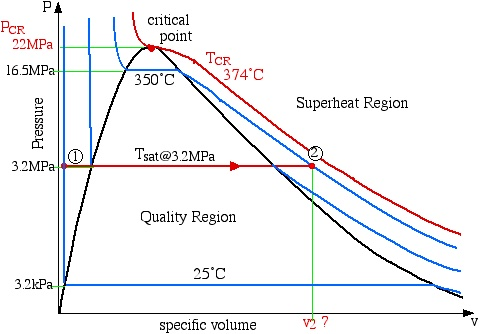
\includegraphics[width=0.75\textwidth]{example2-2_pv}
%\captionof{figure}{State diagram for Example 2.2}
%\label{fig:ch2_example2_diagram}
\end{center}

{\bf Step 3: Address Prompt} \quad As in the previous example, on scanning the superheated tables we find that we need to interpolate between pressure $p$=3.0 MPa and $p$=3.5 MPa in order to determine the specific volume at the required pressure of 3.2 MPa as follows:

\begin{center}
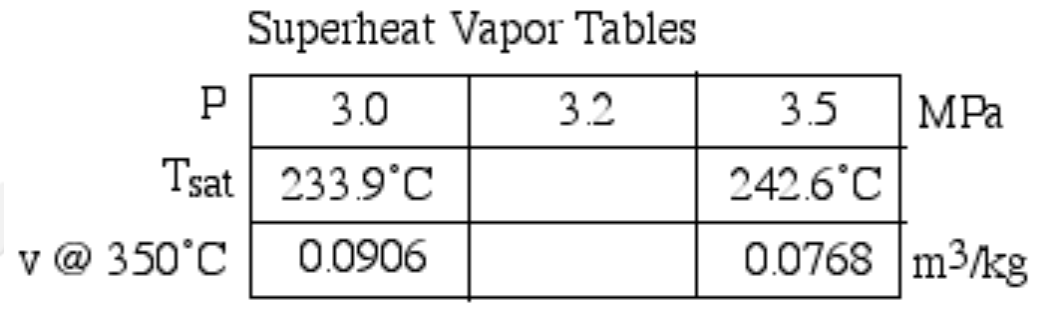
\includegraphics[width=0.6\textwidth]{example2-2_tables}
%\captionof{figure}{State diagram for Example 2.2}
%\label{fig:ch2_example2_diagram}
\end{center}

\begin{equation*}
  \frac{\Delta p_A}{\Delta p_b} = \frac{\Delta v_A}{\Delta v_b} \rightarrow \frac{3.2 - 3.0}{3.5-3.0} = \frac{v_2-0.0906}{0.0768-0.0906} = 0.4
\end{equation*}
Therefore, $v_2 = 0.085 \frac{\rm m^3}{\rm kg}$ and \redbox{V_2 = 0.17\ \rm m^3.}

\end{example}

% --------------------------------------------------------------------
\section{Ideal Gas Equation of State}
% --------------------------------------------------------------------
We find that for a pure substance in the superheated region, at specific volumes much higher than that at the critical point, the $p$-$v$-$T$ relation can be conveniently expressed by the {\bf ideal gas equation of state} to a high degree of accuracy, as follows:
\begin{equation} \label{idealGasLaw}
  p v = R T
\end{equation}
where: $R$ is constant for a particular substance and is called the {\bf gas constant}.

Note that for the ideal gas equation both the pressure $p$ and the temperature $T$ must be expressed in absolute quantities.

The gas constant R can be expressed as follows:

\begin{equation}
  R = \frac{R_u}{M} \left[\frac{\rm kJ}{\rm kg \cdot K}\right]
\end{equation}

where $R_u = 8.314 \frac{\rm kJ}{\rm kmol \cdot K}$, and is known is the {\bf universal gas constant}.  $M$ is the molar mass of the gas, measured in $\left[\frac{\rm kg}{\rm kmol}\right]$ or $\left[\frac{\rm lbm}{\rm lbmol}\right]$ (which yield the same numerical value).
For air,
\begin{equation*}
  M = 28.97 \frac{\rm kg}{\rm kmol} \rightarrow R_{air} = 0.287 \frac{\rm kJ}{\rm kg\cdot K}
\end{equation*}

For water/steam,
\begin{equation*}
  M = 18.02 \frac{\rm kg}{\rm kmol} \rightarrow R_{H_2O} = 0.4615 \frac{\rm kJ}{\rm kg\cdot K}
\end{equation*}

\begin{example}{Checking the Ideal Gas Law}
A piston-cylinder device contains 0.5 kg saturated liquid water at a pressure of 200 kPa. Heat is added and the steam expands at constant pressure until it reaches 300°C.

a) Draw a diagram representing the process showing the initial and final states of the system.

b) Sketch this process on a T-v (temperature-specific volume) diagram with respect to the saturation lines, critical point, and relevant constant pressure lines, clearly indicating the initial and final states.

c) Using steam tables determine the initial temperature of the steam prior to heating.

d) Using steam tables determine the final volume of the steam after heating

e) Using the ideal gas equation of state determine the final volume of the steam after heating. Determine the percentage error of using this method compared to that of using the steam tables.


{\bf Solution:}

Even if questions a) and b) were not required, this should always be the first priority item in solving a thermodynamic problem.

\begin{center}
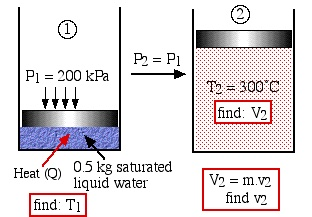
\includegraphics[width=0.5\textwidth]{example2-5_diagram}
%\captionof{figure}{State diagram for Example 2.2}
%\label{fig:ch2_example2_diagram}
\end{center}

\begin{center}
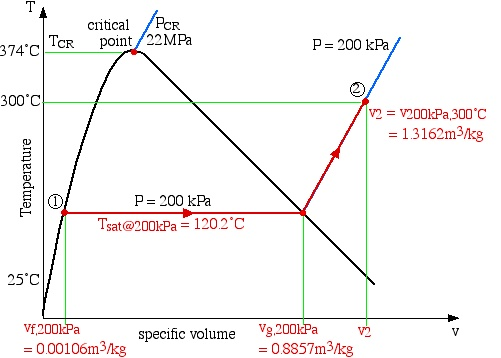
\includegraphics[width=0.5\textwidth]{example2-5_Tv}
%\captionof{figure}{State diagram for Example 2.2}
%\label{fig:ch2_example2_diagram}
\end{center}

c) Since state (1) is specified as saturated liquid at 200 kPa, we use the saturated pressure steam tables to determine that $\redbox{T_1=T_{sat}(200{\rm kPa}) = 120.2°{\rm C}}$.

d) From the $T$-$v$ diagram we determine that state (2) is in the superheated region, thus we use the superheated steam tables to determine that $v_2$ = $v({\rm 200kPa,300°C}$ = 1.3162 m3/kg. Thus $V_2 = m\cdot v_2 = (0.5{\rm kg})\cdot (1.3162 {\rm m^3/kg}) = \redbox{0.658 {\rm m^3}} = 658 {\rm L}$

e) We use $pv = RT$ as our base equation.  Note that pressure and temperature must be absolute!

\begin{equation*}
  v = \frac{RT}{p} \rightarrow v_2 = \frac{0.4615\ {\rm kJ/(kg\cdot K)} \cdot (300 + 273)\ {\rm K}}{200 \rm\ kPa} = 1.322 \frac{\rm m^3}{\rm kg}
\end{equation*}

Therefore, $V_2 = m\cdot v_2 = = (0.5{\rm kg})\cdot (1.322 {\rm m^3/kg}) = \redbox{0.661 {\rm m^3}} = 661 {\rm L}$.

Finally, we calculate error:
\begin{equation*}
  {\rm error} = \left|\frac{\rm true\ value - estimated\ value}{\rm true\ value}\right| = \left|\frac{0.658 - 0.661}{0.658}\right|\approx 0.005 = \redbox{0.5\%}
\end{equation*}

\end{example}

As a side-note, we see the unit ratio $\rm kJ / kPa$ quite often.  Expanding these out results in:
\begin{equation*}
  \frac{\rm kJ}{\rm kPa} = \frac{\rm kN\cdot m}{\rm kN / m^2} = {\rm m}^3
\end{equation*}

\section{Non-Ideal Gas Behavior}
The $T$-$v$ diagram for water is shown below, with the addition of error that arises from calculating the pressure through the ideal gas law.

\begin{figure}[H]
\centering
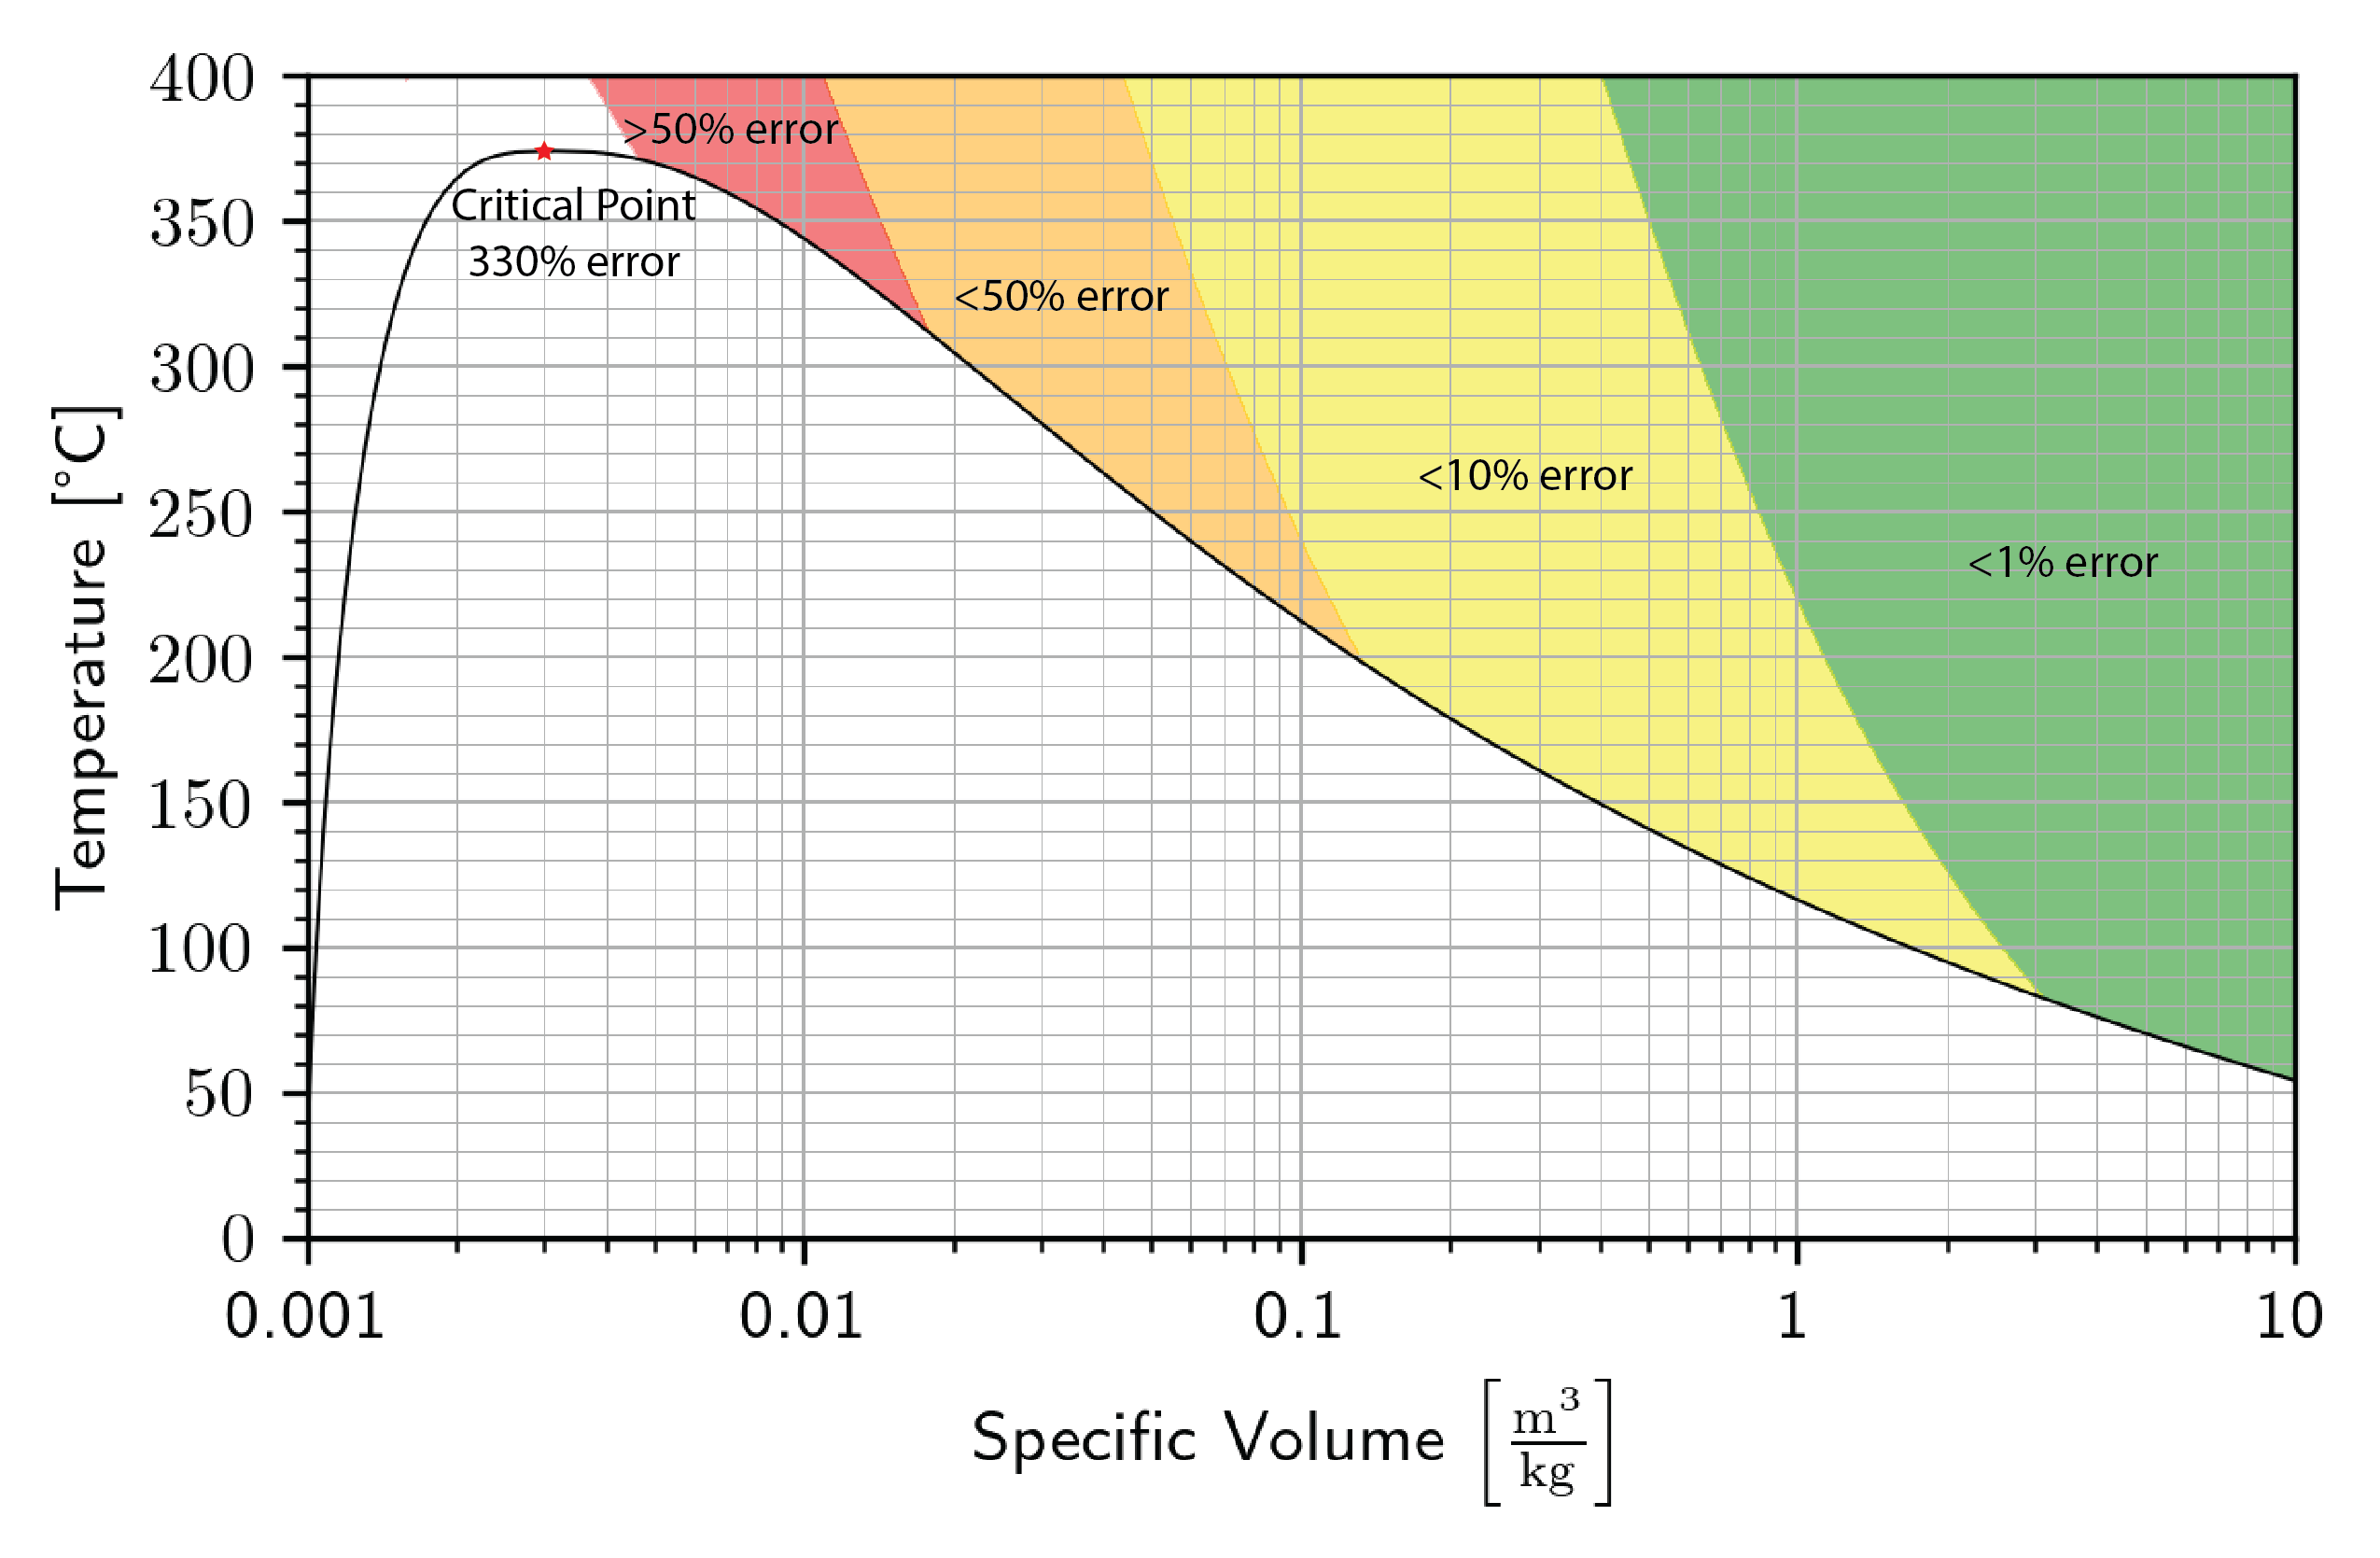
\includegraphics[width=1.0\textwidth]{IdealGasErrorTv}
\caption{$T$-$v$ diagram, including errors from ideal gas equation of state.}
\label{fig:ch2_Tv-ideal}
\end{figure}

Note that error tends to decrease somewhat as temperature increases, but is much more affected by specific volume (and therefore pressure). Note that at the critical point the error is 330\%.  This non-ideal behavior can be accounted for by a correction factor called the {\bf compressibility factor} $Z$ defined as follows:

\begin{equation}
  pv = ZRT \rightarrow Z = \frac{pv}{RT}
\end{equation}

When the compressibility factor Z approaches 1, the gas behaves as an ideal gas. By specifying both temperature and pressure, the compressibility factor can be expressed as:

\begin{equation} \label{eq:ch2_Zdef}
  Z = \frac{v_{actual}}{v_{ideal}}
\end{equation}

All fluids normalized in this manner exhibit similar non-ideal gas behavior within a few percent, thus they can all be plotted on a Generalized Compressibility Chart. A number of these charts are available, however we prefer to use the Lee-Kesler (logarithmic) Compressibility Chart, shown below.


\begin{figure}[H]
\centering
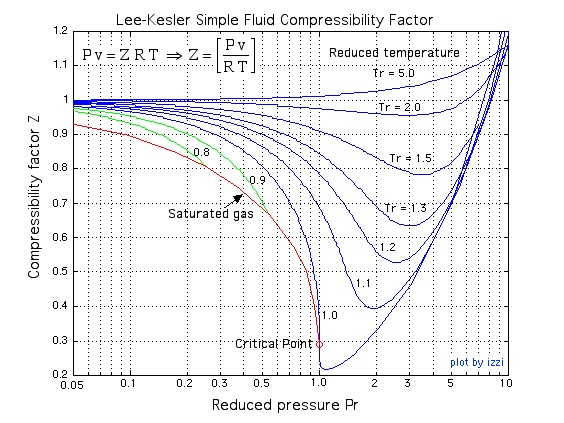
\includegraphics[width=0.75\textwidth]{Zfactor}
\caption{Compressibility factor for non-ideal gases.}
\label{fig:ch2_Zfactor}
\end{figure}

Notice that the compressibility factor is dependent on the reduced pressure and temperature.  These are defined as follows:
\begin{align}
  p_R &= \frac{p}{p_{crit}} &   T_R &= \frac{T}{T_{crit}}
\end{align}

Different fluids have different values of critical point pressure and temperature data $p_{crit}$ and $T_{crit}$, and these can be determined from the Table of Critical Point Data of Various Substances in Appendix \ref{sec:idealGasProps}.

\begin{example}[label={ex:ch2idealGas}]{Correcting the Ideal Gas Law}
  Carbon Dioxide gas is stored in a 100 liter tank at 6 MPa and 30°C. Determine the mass of $\rm CO_2$ in the tank based on (a) the ideal gas equation of state, (b) the generalized compressibility chart, and (c) values obtained from the $\rm CO_2$ tables of data.  Determine the percentage error in each case.

  {\bf Solution Approach:}

  There is only one state here, so there is little to gain by drawing the state diagrams.  Likewise, the $T-v$ diagram is useful when using tables, but we want to use the ideal gas law for our calculations.

  For $\rm CO_2$, the molar mass is $M = 44.01 \frac{\rm kg}{\rm kmol}$, which leads to a gas constant of $R_{CO_2}=0.1889 \frac{\rm kJ}{\rm kg\cdot K}$.  We can use this in the ideal gas equation of state:

  \begin{equation*}
    v_{ideal} = \frac{R\cdot T}{p} = \frac{0.1889 \frac{\rm kJ}{\rm kg\cdot K} \cdot 303\ {\rm K}}{6000\ {\rm kPa}}= 0.00954 \frac{\rm m^3}{\rm kg}
  \end{equation*}

  Mass can then be found from the equation $V = m \cdot v$:
  \begin{equation*}
    m_{ideal} = \frac{V}{v} = \frac{100\ \rm L}{0.00954 \frac{\rm m^3}{\rm kg}} \cdot \frac{1\ \rm m^3}{1000\ \rm L} \rightarrow \redbox{m_{ideal} = 10.5\ {\rm kg}}
  \end{equation*}
  
  To use the compressibility chart, we need to find the critical temperature and pressure for $\rm CO_2$.  This comes from the Table of Critical Point Data of Various Substances (Appendix \ref{sec:idealGasProps}): $p_{crit} = 7.39\ {\rm MPa}$, $T_{crit} = 304.2\ K$.

  Next, we calculate our reduced temperature and pressure:
  \begin{align*}
    p_R = \frac{p}{p_{crit}} &= \frac{6\rm\ MPa}{7.39\rm\ MPa} = 0.81 \\
    T_R = \frac{T}{T_{crit}} &= \frac{30 + 273.15\rm\ K}{304.2\rm\ K} \approx 1.0 \\
  \end{align*}

With our reduced pressure and temperature in hand, we go to the compressibility factor chart.  We start at our pressure on the x-axis, shoot a line up until we hit our desired reduced temperature line, then the y-axis position of that point will be our $Z$ value.
  
\begin{center}
\includegraphics[width=0.75\textwidth]{example2-4_CO2Comp}
%\captionof{figure}{State diagram for Example 2.2}
%\label{fig:ch2_example2_diagram}
\end{center}

Since $Z=0.62$, we can use Equation \ref{eq:ch2_Zdef}:
\begin{equation*}
  Z = \frac{v_{comp}}{v_{ideal}} \rightarrow v_{comp} = 0.62 \cdot 0.00954 \frac{\rm m^3}{\rm kg} = 0.00591 \frac{\rm m^3}{\rm kg}
\end{equation*}

Mass is found the same way as before:
\begin{equation*}
    m_{comp} = \frac{V}{v} = \frac{100\ \rm L}{0.00591 \frac{\rm m^3}{\rm kg}} \cdot \frac{1\ \rm m^3}{1000\ \rm L} \rightarrow \redbox{m_{comp} = 16.9\ {\rm kg}}
\end{equation*}

Finally, we'll get the most accurate answer from the $\rm CO_2$ tables:
\begin{equation*}
  v_{actual} = 0.005833 \frac{\rm m^3}{\rm kg} \rightarrow \redbox{m_{actual} = 17.14 kg}
\end{equation*}

This means that the compressibility chart had an error of about 1\% (mostly due to the inaccuracy of reading charts). The ideal gas law without a compressibility correction had an error of around 39\%!

\end{example}


% --------------------------------------------------------------------
\section{Using Software: Google Colab (Python) with CoolProp} \label{sec:ch2_colab}
% --------------------------------------------------------------------
As we saw in Section \ref{sec:ch1_colab}, \href{https://colab.research.google.com}{Google Colab} is a free IDE (integrated development environment) for Python.  Through Colab, you can write Python code, link to countless existing libraries of code and data, and run the code you write.

Hopefully, you already have a basic understanding of how to use Python for your homework.  In this section, we will be using a library called \href{http://www.coolprop.org/}{CoolProp} to determine the properties of materials, instead of looking up values from tables.

\subsection{Setup and CoolProp Basics}
First off, in order to access the CoolProp library, we need to input the line

\begin{verbatim}
!pip install CoolProp
\end{verbatim}

This tells Google Colab that we plan on using the library, and it should expect to link to it later.

In a separate cell (which is created using the ``+ Code'' button at the top left), you should include the following lines:

\begin{Verbatim}[commandchars=\\\{\}]
\textcolor{OliveGreen}{# Clear all variable definitions}
\textcolor{blue}{\%reset} -f                         
\textcolor{violet}{from} numpy \textcolor{violet}{import} *               \textcolor{OliveGreen}{# Import common numerical functions (like sqrt)}
\textcolor{violet}{from} matplotlib.pyplot \textcolor{violet}{import} *   \textcolor{OliveGreen}{# Import plotting functions (like plot)}
\textcolor{violet}{import} CoolProp.CoolProp \textcolor{violet}{as} CP    \textcolor{OliveGreen}{# Import CoolProp library}
\end{Verbatim}

The only new line in these commands in the ``import CoolProp'' line, which simply links to the CoolProp library.  The phrasing we used means that we need to add ``\texttt{CP.}'' in front of any CoolProp commands we end up using.  If you want to avoid this, you can type ``\texttt{from CoolProp.CoolProp import *}'' instead.  In order to match the rest of the example, I would suggest leaving it as written.

You can now run the two cells by clicking the ``play'' button that appears at the top left of each cell.  You can also run all of the cells in the script by clicking ``Runtime'' from the top menu, then selecting ``Run all''.

\subsection{A Simple Example}

At this point, we are ready to build our first bit of code.  Let's start by reworking Example \ref{ex:ch2idealGas}.

We can calculate the ideal specific volume with the following lines of code:
\begin{Verbatim}[commandchars=\\\{\}]
R = \textcolor{JungleGreen}{8.31446}            \textcolor{OliveGreen}{# Universal Gas Constant (in kJ/kgK)}
M = \textcolor{JungleGreen}{44.01}              \textcolor{OliveGreen}{# Molar Mass of CO2}
RCO2 = R/M             \textcolor{OliveGreen}{# CO2 gas constant}
p = \textcolor{JungleGreen}{6000}               \textcolor{OliveGreen}{# pressure in kPa}
T = \textcolor{JungleGreen}{30} + \textcolor{JungleGreen}{273.16}        \textcolor{OliveGreen}{# Conversion of temperature from Celsius to Kelvin}
vIdeal = RCO2 * T / p  \textcolor{OliveGreen}{# Ideal Gas Law solved for v}
print(\textcolor{purple}{'Ideal v = '}, vIdeal, \textcolor{purple}{'m^3/kg'})   
\end{Verbatim}
Note that the \texttt{print} statement at the end is needed to see the results:
\begin{Verbatim}
Ideal v =  0.009545602111641295 m^3/kg
\end{Verbatim}
You can use the simpler \texttt{print(vIdeal)} as a shortcut, which will only print the number.  However, with multiple print statements, you can lose track of the meanings of the numbers, which is I prefer the slightly longer version used above.

\subsection{Using CoolProp}
The general form of the CoolProp function is as follows:
\begin{Verbatim}[commandchars=\\\{\}]
<outputVariable> = CP.PropsSI(<outputType>, <input1Type>, <input1Value>,
<input2Type>, <input2Value>, <materialName>)
\end{Verbatim}
You can see the full list of Types \href{http://www.coolprop.org/coolprop/HighLevelAPI.html#table-of-string-inputs-to-propssi-function}{online}, or you can use the short list below:
\begin{table}[H]
  \centering
  \caption{List of CoolProp Types and Meanings}
  \label{tab:ch2_CoolProp}
  \begin{tabular}{cl}
  Type & Meaning \\ \hline
  \texttt{'D'} & Density [kg/$\rm m^3$]\\
  \texttt{'H'} & Enthalpy [J/kg]\\
  \texttt{'P'} & Pressure [Pa]\\
  \texttt{'Q'} & Quality  [-]\\
  \texttt{'S'} & Entropy  [J/kgK]\\
  \texttt{'T'} & Temperature [K]\\
  \texttt{'U'} & Internal Energy [J/kg]
  \end{tabular}
\end{table}

Unfortunately, there is no option for specific volume.  Instead, we must use the identity that $v = 1/{\rho}$ to switch between density and specific volume.
Using this identity, the second half of Example \ref{ex:ch2idealGas} can be recreated using the CoolProp library:
\begin{Verbatim}[commandchars=\\\{\}]
p = \textcolor{JungleGreen}{6000}*\textcolor{JungleGreen}{1000}          \textcolor{OliveGreen}{# Conversion of pressure from kPa to Pa}
T = \textcolor{JungleGreen}{30} + \textcolor{JungleGreen}{273.16}        \textcolor{OliveGreen}{# Conversion of temperature from Celsius to Kelvin}
dActual = CP.PropsSI(\textcolor{purple}{'D'}, \textcolor{purple}{'P'}, p, \textcolor{purple}{'T'}, T, \textcolor{purple}{'CO2'})
vActual = \textcolor{JungleGreen}{1}/dActual
print(\textcolor{purple}{'Actual v = '}, vActual, \textcolor{purple}{'m^3/kg'})   
\end{Verbatim}

Note the conversion necessary for pressure (from kPa to Pa), as well as the conversion for temperature (from Celsius to Kelvin).  This code has the following output:
\begin{Verbatim}
Actual v =  0.005833989613407337 m^3/kg
\end{Verbatim}
The difference between this result and Example \ref{ex:ch2idealGas} stems from the inaccuracy of reading from a plot.

\subsection{Exporting from Colab as a PDF}
You can create a PDF of your code, including the output, by clicking the ``File'' menu option and navigating to ``Print'' at the bottom.

In the dialog that pops up, choose ``Save as PDF'' in the Destination drop-down menu, then click save.  The resulting PDF for the work above is shown in Figure \ref{fig:ch2_Colab}.

\begin{figure}[H]
\centering
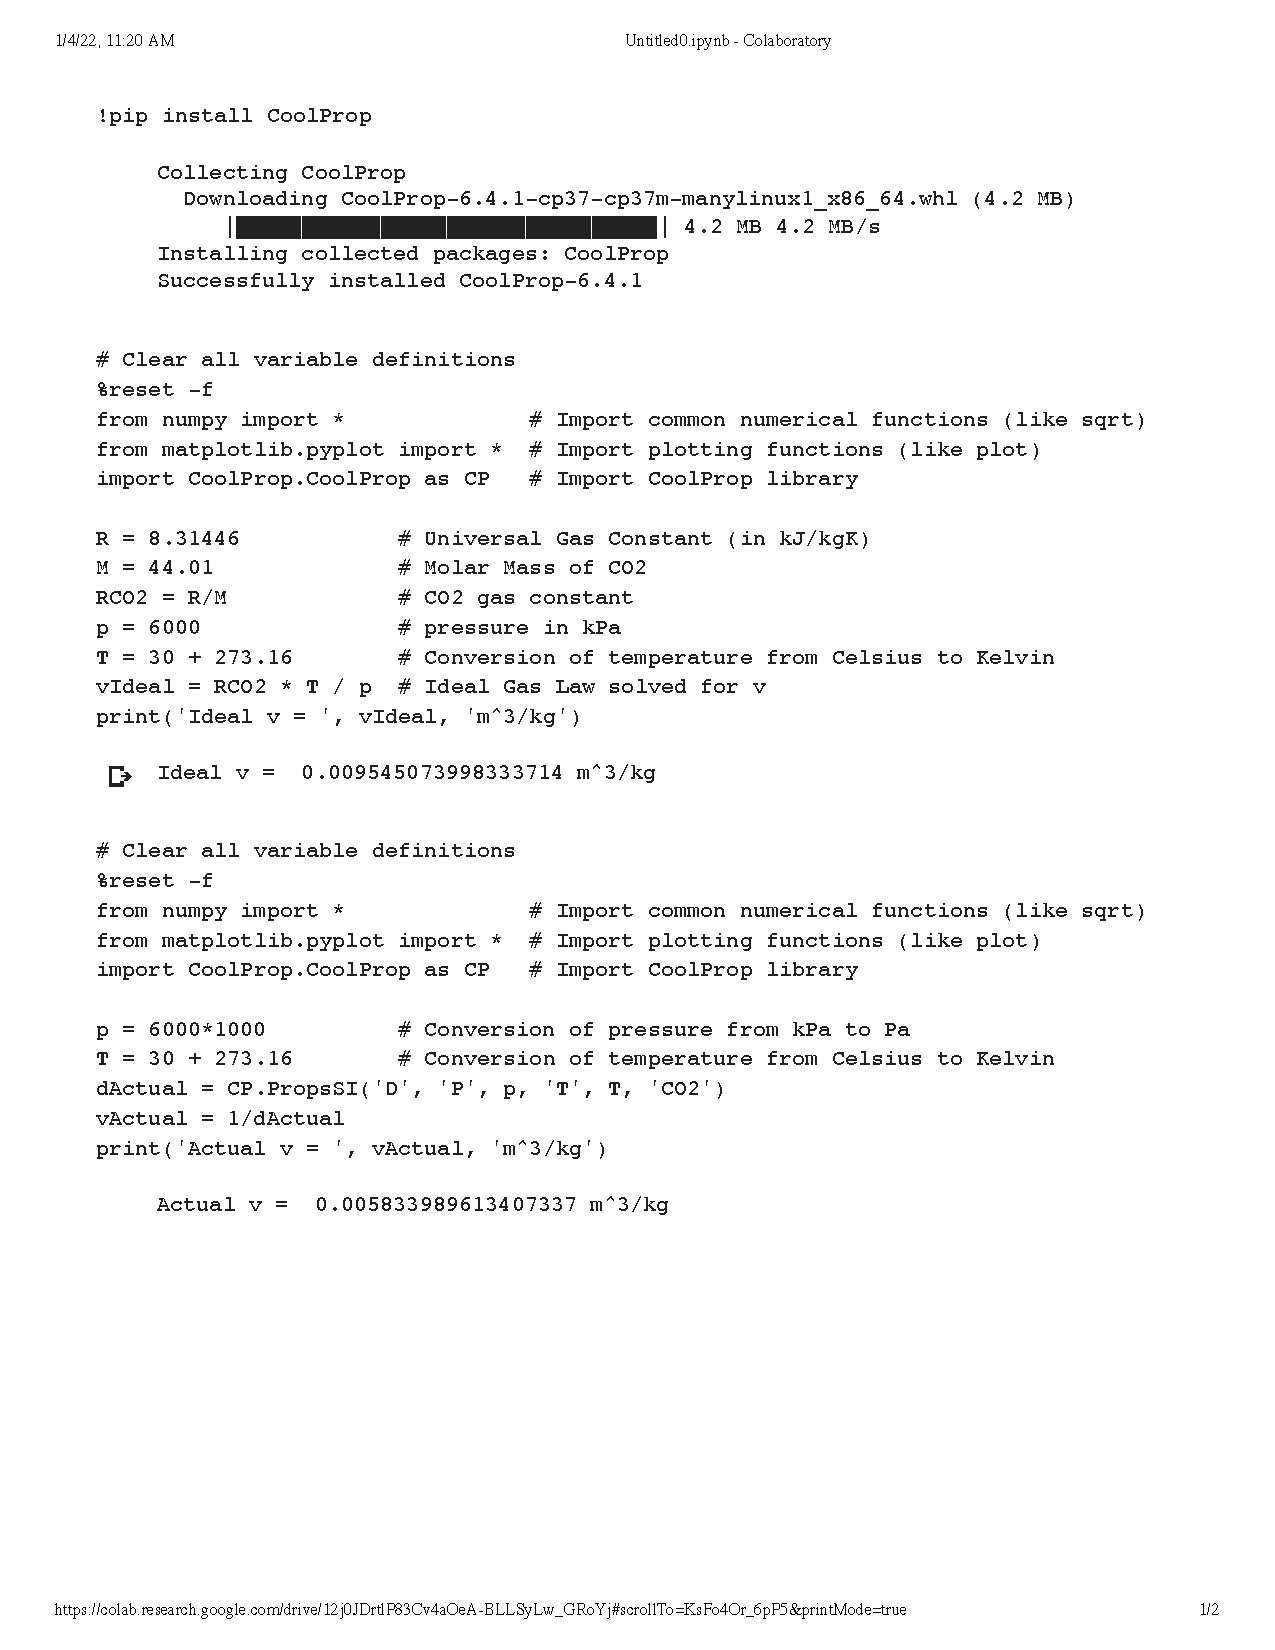
\includegraphics[width=0.75\textwidth]{ColabExample}
\caption{Output from Google Colab saved as a PDF.}
\label{fig:ch2_Colab}
\end{figure}


% --------------------------------------------------------------------
\section{Summary}
% --------------------------------------------------------------------

In this chapter, we determined the state of matter, which was determined by two independent properties, and then used that state to determine any missing properties.  As part of this process, we introduced linear interpolation to find values from the table that are not explicitly listed.  We also considered a number of processes, which are simply the change between two states.

Finally, we looked at two alternatives to the steam tables: the ideal gas law and software.  The ideal gas law requires a lot more calculation, but can be used when the steam tables are not available (which is typically the case).  Most importantly, a compressibility correction is necessary for low temperatures and/or high pressures.  Software can be used in most circumstances, but experience in coding is necessary to obtain accurate solutions.

\begin{homework}
  %--------------------------------------------------------------------
  \question How many independent quantities are necessary to fully describe a state of matter?
  %--------------------------------------------------------------------
  \question Define the following: phase, state, property, process
  %--------------------------------------------------------------------
  \question Two kilograms of water at 25°C are placed in a piston cylinder device under 3.2 MPa pressure. Heat is added to the water at constant pressure until the temperature of the fluid reaches 350°C (State (2)). Determine the final volume of the fluid at state (2). $\answer{[0.08508\ {\rm m^3}/{\rm kg}]}$
   %--------------------------------------------------------------------
  \question A piston-cylinder device contains a saturated mixture of steam and water having a total mass of 0.5 kg at a pressure of 160 kPa and an initial volume of 100 liters. Heat is then added and the fluid expands at constant pressure until it reaches a saturated vapor state.
\begin{questionparts}
\item Draw a diagram representing the process showing the initial and final states of the system.

\item Sketch this process on a P-v diagram with respect to the saturation lines, critical point, and relevant constant temperature lines, clearly indicating the initial and final states.

\item Determine the initial quality and temperature of the fluid mixture prior to heating. {\color{red} [$x_1$ = 0.182, $T_1$ = 113.3°C]}

\item Determine the final volume of the steam after heating. {\color{red} [0.546 $\rm m^3$ (546 liters)]}
\end{questionparts}
%--------------------------------------------------------------------
\question A pressure cooker allows much faster (and more tender) cooking by maintaining a higher boiling temperature of the water inside. It is well sealed, and steam can only escape through an opening on the lid, on which sits a metal petcock. When the pressure overcomes the weight of the petcock, the steam escapes, maintaining a constant high pressure while the water boils.

\begin{center}
  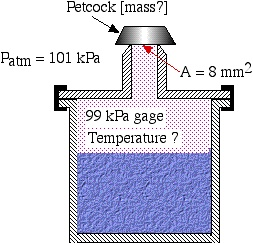
\includegraphics[width=0.4\textwidth]{press_cooker}
\end{center}
  
Assuming that the opening under the petcock has an area of 8 $\rm mm^2$, determine:

\begin{questionparts}
\item the mass of the petcock required in order to maintain an operating pressure of 99 kPa gauge. {\color{red}[80.7 g]}

\item the corresponding temperature of the boiling water. {\color{red}[120.2°C]}
\end{questionparts}
Note: Assume that the atmospheric pressure is 101 kPa. Draw a free body diagram of the petcock.

%--------------------------------------------------------------------
\question Consider a rigid container having a volume of 100 liters, filled with steam at an initial state of 400 kPa and 300°C. The steam is then cooled until it reaches a temperature of 90°C.

\begin{questionparts}
\item Draw a diagram representing the process showing the initial and final states of the system.

\item Using steam tables determine the mass of steam in the container. {\color{red} [0.153 kg]}

\item Using the ideal gas equation of state determine the mass of steam in the container. {\color{red} [0.151 kg]}
Determine the percentage error of using this method compared to that of using the steam tables. {\color{red}[1\%]}

\item Sketch this process on a $T$-$v$ (temperature-specific volume) diagram with respect to the saturation lines, critical point, and relevant constant pressure lines, clearly indicating the initial and final states.

\item Using steam tables determine the final pressure and quality of the fluid mixture after cooling. {\color{red}[70.2 kPa, $x$ = 0.277]}
\end{questionparts}
Note: The critical point data and ideal gas constant for steam can be found on the first page of the steam tables.

%--------------------------------------------------------------------

\question An automobile tire with a volume of 100 liters is inflated to a gauge pressure of 210 kPa. Determine:
\begin{questionparts}
\item the mass of air in the tire if the temperature is 20°C {\color{red} [$m$ = 0.369 kg]}
\item the increase in gauge pressure if the temperature in the tire reaches 50°C \\{\color{red} [$p_{2,gage}=$242 kPa]}
\end{questionparts}
Assume that atmospheric pressure is 100 kPa.

%--------------------------------------------------------------------

\question Compressed air is commonly used to power a large variety of power tools.  Lowe's sells an air compressor that can fill an 8-gallon tank to 160 psi. At a temperature of 70°F, determine the mass of the air inside a full 8-gallon tank.  Let $p_{atm} = 14.7$ psi.
\begin{questionparts}

\item Use the ideal gas law (you will need to do a lot of unit conversions for this). \\{\color{red} [0.429 kg]}

\item Find the compressibility factor.  How far off is your analysis above? {\color{red} [0.99]}

\end{questionparts}
\end{homework}

